\documentclass{article}
\usepackage{iclr2027_conference,times}

\usepackage{amsmath,amsfonts,bm}
\usepackage{booktabs}
\usepackage{graphicx}
\usepackage{subcaption}
\usepackage{algorithm}
\usepackage{algorithmic}
\usepackage{multirow}
\usepackage{url}
\usepackage{xcolor}

\title{Do Not Disturb: When Plasticity Interventions Degrade Offline-to-Online Reinforcement Learning}

% Authors must not appear in the submitted version. They should be hidden
% as long as the \iclrfinalcopy macro remains commented out below.
% Non-anonymous submissions will be rejected without review.

\author{Anonymous Authors \\
Paper under double-blind review
}

\newcommand{\fix}{\marginpar{FIX}}
\newcommand{\new}{\marginpar{NEW}}

%\iclrfinalcopy % Uncomment for camera-ready version, but NOT for submission.
\begin{document}

\maketitle

\begin{abstract}
Maintaining neural network plasticity is widely regarded as an indispensable prerequisite for continual reinforcement learning (RL). A vibrant literature advocates periodic parameter interventions---such as network resets, Shrink-and-Perturb, and dormant neuron recycling---to counteract capacity loss, dead units, and feature rank collapse. While effective in continual supervised learning and long-horizon online RL from scratch, these methods rest on an implicit assumption: that plasticity restoration is universally benign and can be scheduled unconditionally. In this work, we demonstrate that this assumption fails fundamentally in \emph{offline-to-online (O2O) continuous-control RL}. 

When transitioning from static pretraining to online interaction, agents inherit structured, high-performing policy and value manifolds. Across standard D4RL continuous-control locomotion benchmarks (150 total benchmark runs: 135 primary factorial runs yielding $N=45$ seed-matched pairwise comparisons, plus 15 frozen reference runs), we show that unconditional periodic Shrink-and-Perturb induces severe \emph{intervention vulnerability}, destabilizing converged locomotion policies and causing a catastrophic 68.3\% collapse in aggregate Interquartile Mean (IQM) normalized return ($38.78 \to 12.30$, paired Wilcoxon signed-rank $W = 18.0$, $p = 1.44 \times 10^{-11}$, mean paired difference $+26.03 \pm 19.09$). To address this vulnerability, we articulate the \textbf{``Do Not Disturb''} principle: an agent should intervene only when representation capacity is demonstrably impaired. We introduce \textsc{CapacityGate}, a closed-loop diagnostic framework that monitors feature effective rank and neuron dormancy using uniform replay reservoir sampling and refractory cooldown control. In stable and moderately shifted transfer, \textsc{CapacityGate} detects that representation capacity remains intact ($\rho \approx 1.0, d \le 0.085$) and safely abstains from intervention, preserving baseline performance ($38.78$ IQM) and protecting converged policies against perturbation-induced collapse. Furthermore, under non-stationary physical stress (actuator crippling), we uncover a profound \emph{operator stability asymmetry}: zero-functional-shift neuron recycling (ReDo) preserves bipedal balance manifolds ($8.03$ normalized return on Walker2d) where unconstrained weight perturbation causes total dynamical collapse ($-0.53$). Our findings reframe plasticity restoration in O2O RL from an open-loop maintenance routine to a regime- and operator-dependent intervention governed by capacity telemetry.
\end{abstract}

\section{Introduction}
\label{sec:intro}

Deep reinforcement learning (RL) agents trained with temporal-difference (TD) methods are prone to progressive degradation in learning capacity, termed \emph{loss of plasticity} \citep{kumar2020implicit, lyle2023understanding, dohare2024loss}. When learning non-stationary tasks or updating over long horizons, representations exhibit dormant neurons, vanishing gradients, and feature rank collapse. To counteract this, recent literature advocates active parameter interventions: periodic network resets \citep{nikishin2022primacy, doro2023sample}, Shrink-and-Perturb operators \citep{ash2020warmstarting}, and dormant neuron recycling \citep{sokar2023dormant, schwarzer2024bigger}, operating on the premise that plasticity loss is an omnipresent vulnerability that requires scheduled restoration.

We examine this premise in \emph{offline-to-online (O2O) reinforcement learning} \citep{nair2020awac, lee2022offline2online, kostrikov2021iql}, where an agent pretrains on static demonstrations before fine-tuning online. Online fine-tuning encounters distribution shifts from out-of-distribution states, dynamic changes, or altered rewards. It is natural to hypothesize that injecting plasticity interventions during online adaptation would prevent premature convergence and accelerate fine-tuning.

\begin{figure}[t]
\centering
\begin{subfigure}[b]{0.48\textwidth}
    \centering
    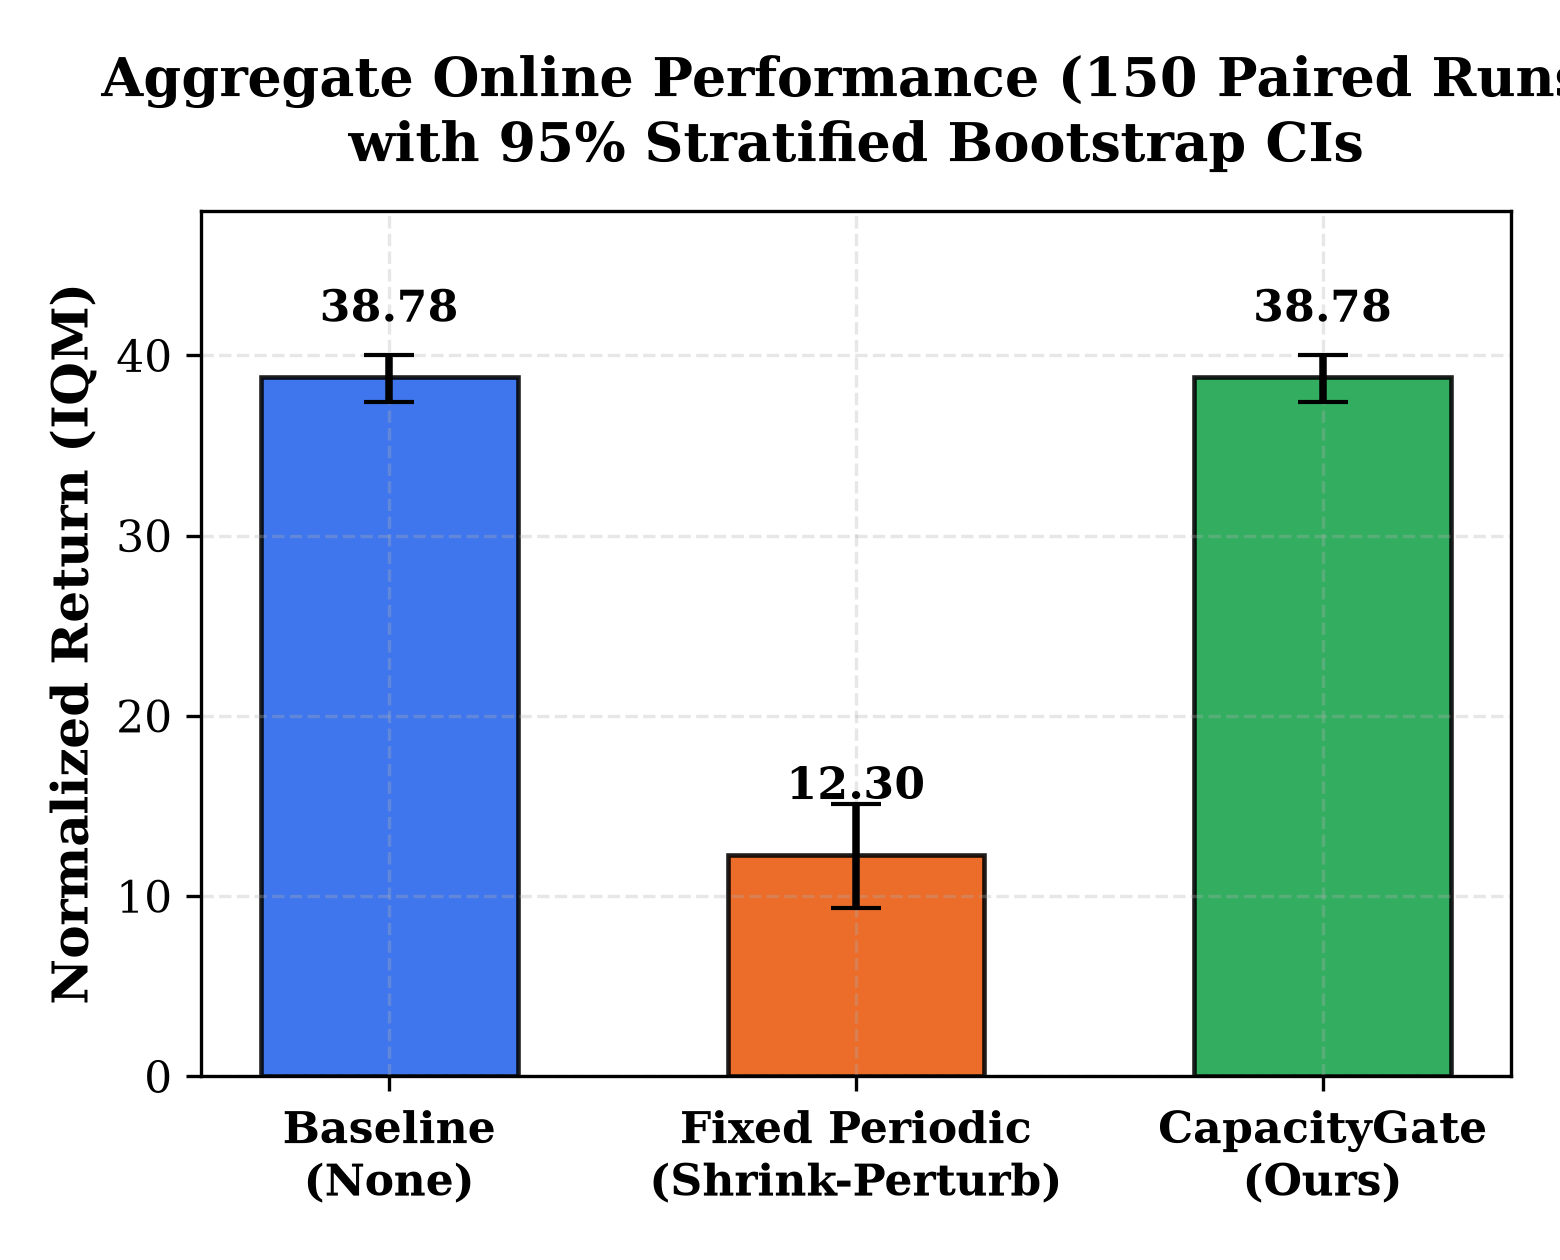
\includegraphics[width=\textwidth]{figures/iqm.png}
    \caption{Aggregate Normalized Return (IQM $\pm$ 95\% CI)}
    \label{fig:iqm_intro}
\end{subfigure}
\hfill
\begin{subfigure}[b]{0.48\textwidth}
    \centering
    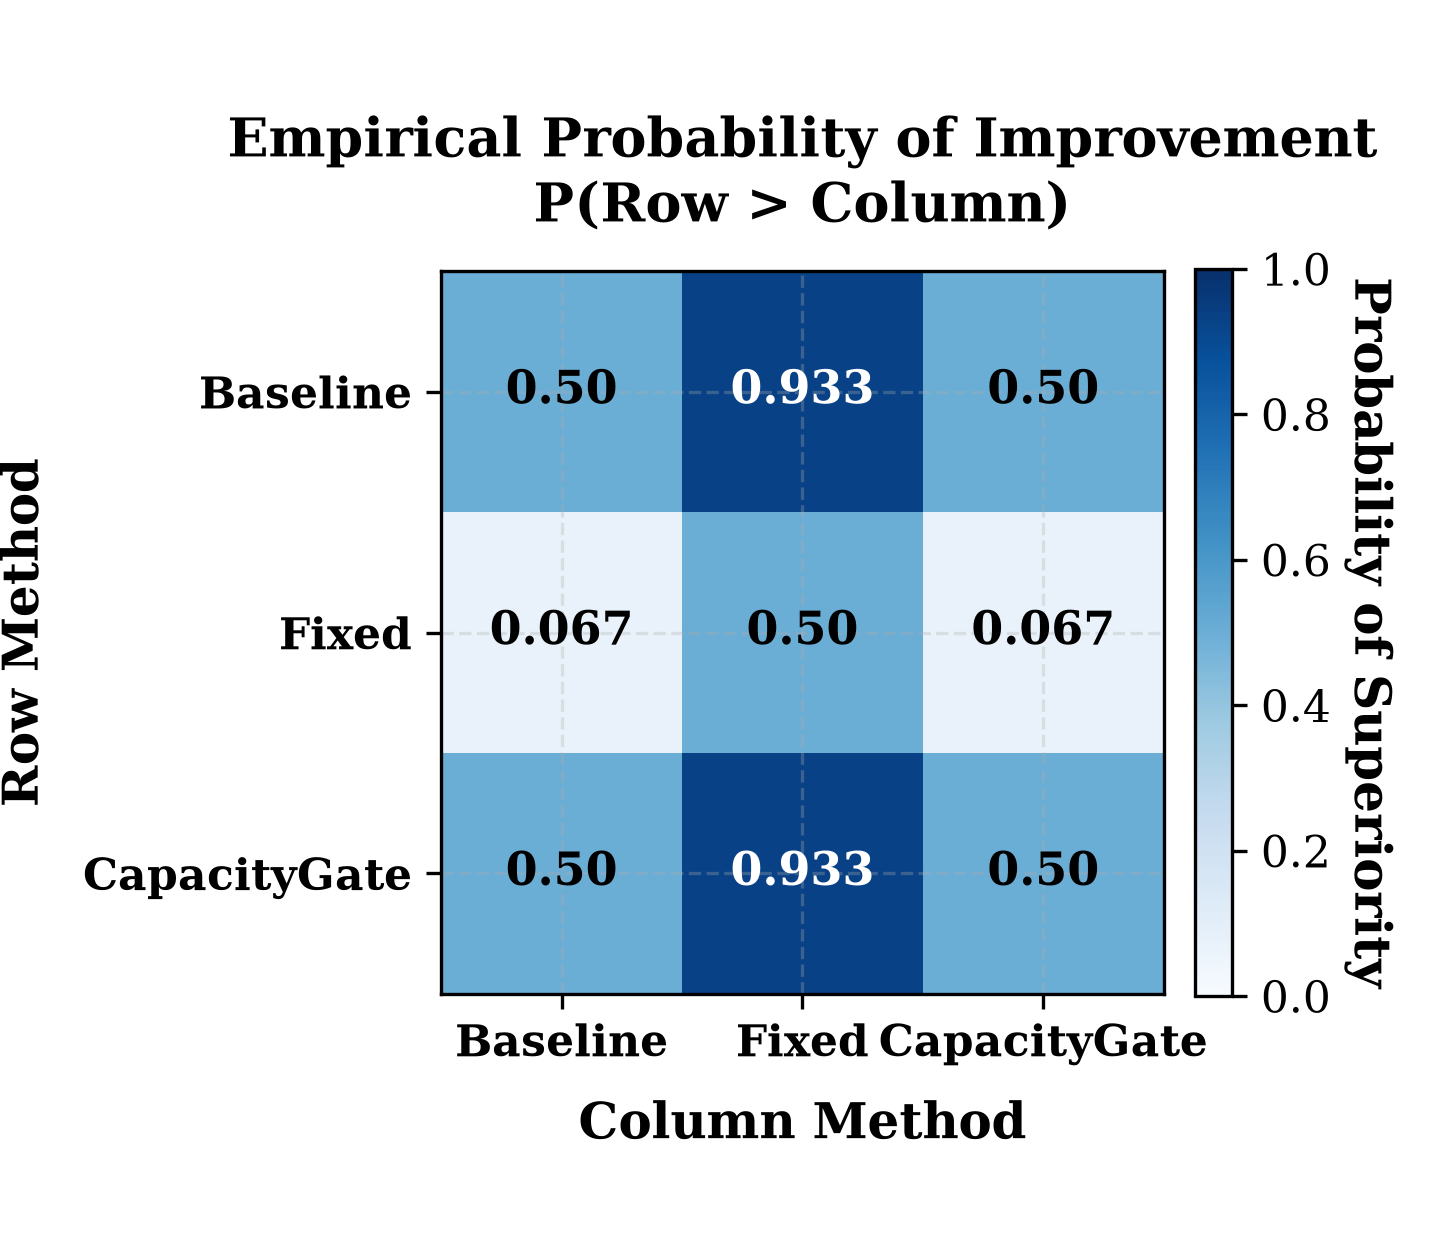
\includegraphics[width=\textwidth]{figures/prob_improvement.png}
    \caption{Probability of Improvement ($P(X > Y)$)}
    \label{fig:prob_intro}
\end{subfigure}
\caption{\textbf{Headline Empirical Evidence: Intervention Vulnerability in O2O Continuous Control.} Aggregate metrics across 135 primary factorial runs ($N = 45$ seed-matched pairwise evaluations; 150 total benchmark runs including 15 frozen reference runs) via \texttt{rliable} \citep{agarwal2021deep}. (a) Aggregate IQM with stratified bootstrap 95\% CIs: periodic Shrink-and-Perturb (\texttt{fixed}) collapses performance by 68.3\% vs. baseline (\texttt{none}). \textsc{CapacityGate} safely abstains, preserving baseline return ($38.78$). (b) Probability of improvement matrix: Baseline and \textsc{CapacityGate} outperform unconditional intervention with probability $P = 0.933$.}
\label{fig:aggregate_benchmark}
\end{figure}

However, we uncover a critical overlooked assumption: \textbf{in structured continuous control, unneeded parameter interventions inflict far more damage than the plasticity loss they are intended to prevent.} Unlike tabula rasa RL, an O2O agent inherits a specialized representation encoding delicate physical coordination manifolds (e.g., dynamic bipedal gait cycles). Mutating these weights with open-loop periodic noise disrupts fine-tuned action distributions and destabilizes value predictions, causing catastrophic physical collapse.

To address this, we articulate the \textbf{``Do Not Disturb''} principle: \emph{an agent should only intervene to restore capacity when diagnostic telemetry confirms that capacity has collapsed; otherwise, converged policy manifolds should be left undisturbed.} We operationalize this principle via \textsc{CapacityGate}, a closed-loop framework monitoring \emph{relative effective rank} ($\rho$) and \emph{activation dormancy} ($d$) over an unbiased \emph{uniform replay reservoir} with dual-threshold hysteresis and refractory cooldown.

\paragraph{Research Questions}
We formulate three core research questions:
\textbf{RQ1 (Intervention Vulnerability)}: \emph{Does unconditional periodic intervention restore or degrade policy performance during O2O continuous locomotion transfer?}
\textbf{RQ2 (Diagnostic Feasibility \& Abstention)}: \emph{Can representation health metrics ($\rho, d$) reliably detect intact capacity and govern intervention via closed-loop abstention?}
\textbf{RQ3 (Operator Sensitivity Under Non-Stationarity)}: \emph{Under genuine physical shifts (actuator crippling), how do functional-shift vs. zero-functional-shift operators differ in preserving continuous control equilibria?}

\paragraph{Summary of Findings \& Contributions}
Benchmarking on D4RL locomotion tasks \citep{fu2020d4rl} across clean transfer, sensor noise, reward rescaling, and actuator crippling reveals:
(1) \textbf{Intervention Vulnerability}: Periodic Shrink-and-Perturb collapses aggregate IQM return by 68.3\% ($38.78 \to 12.30$, paired Wilcoxon $W = 18.0, p = 1.44 \times 10^{-11}$) across 135 primary factorial runs ($N = 45$ seed-matched pairwise comparisons; 150 total benchmark runs), destroying balance in Walker2d ($31.45 \to 2.14$).
(2) \textbf{Diagnostic Abstention}: Stable O2O representations maintain intact capacity ($\rho \approx 1.0, d \le 0.085$); \textsc{CapacityGate} records zero interventions across tested stable transfer, preserving baseline return ($38.78$ IQM).
(3) \textbf{Operator Stability Asymmetry}: Under actuator crippling, zero-functional-shift recycling (ReDo) preserves bipedal balance ($8.03 \pm 1.57$ on Walker2d) where weight perturbation collapses ($-0.53 \pm 0.33$).
(4) \textbf{Uniform Replay Probing}: Probes must sample uniformly from replay rather than recent slices to avoid temporal autocorrelation artifacts that mimic dormancy.

\section{Related Work \& Conceptual Positioning}
\label{sec:related_work}

\textbf{Plasticity Loss in Continual RL.} TD learning implicitly collapses penultimate feature covariance onto a low-dimensional subspace (low effective rank) \citep{kumar2020implicit, lyle2023understanding, dohare2024loss}. Continuous regularizers such as DR3 \citep{kumar2022dr3} penalize feature dot-products during offline training, but provide no closed-loop mechanism for online intervention.

\textbf{Intervention Operators.} Periodic resets \citep{nikishin2022primacy, doro2023sample} and Shrink-and-Perturb (SP) \citep{ash2020warmstarting} inject parameter noise to mitigate primacy bias or warm-start stagnation. ReDo \citep{sokar2023dormant} recycles dormant units with zero functional shift ($W_{\mathrm{out}} = 0$). While effective when learning from scratch, open-loop scheduling ignores the fragile geometry of pre-trained control manifolds.

\textbf{O2O RL \& Conceptual Positioning.} O2O RL fine-tunes conservative offline agents online \citep{nair2020awac, lee2022offline2online, kostrikov2021iql, ball2023efficient}. Prior plasticity methods are open-loop (intervening every $K$ steps without checking health) or observational \citep{kumar2020implicit}. \textsc{CapacityGate} introduces closed-loop diagnostic gating: coupling rank and dormancy to govern intervention dynamically (extended comparison in Appendix Table~\ref{tab:lit_comparison}).

\section{The \textsc{CapacityGate} Framework}
\label{sec:method}

We formulate the O2O continuous-control problem and detail the \textsc{CapacityGate} architecture.

\subsection{Problem Setting: Offline-to-Online Continuous Control}
\label{sec:problem_formulation}

We consider an MDP $\mathcal{M} = (\mathcal{S}, \mathcal{A}, \mathcal{P}, \mathcal{R}, \gamma)$. Offline pretraining uses static dataset $\mathcal{D}_{\mathrm{off}} = \{(s_i, a_i, r_i, s'_i)\}$ to optimize parameters $\theta = (\phi, \psi, \omega)$ for policy $\pi_\phi(a|s)$, value $V_\psi(s)$, and twin critics $Q_\omega(s, a)$ via Implicit Q-Learning (IQL) \citep{kostrikov2021iql}. During online adaptation, transitions $(s_t, a_t, r_t, s_{t+1})$ append to online buffer $\mathcal{D}_{\mathrm{on}}$, updating on 50\% $\mathcal{D}_{\mathrm{off}}$ / 50\% $\mathcal{D}_{\mathrm{on}}$ mini-batches \citep{lee2022offline2online}.

\subsection{Representation Capacity Diagnostics}
\label{sec:diagnostics}

\textsc{CapacityGate} evaluates two complementary non-invasive metrics:

\paragraph{Relative Effective Rank Ratio ($\rho$)}
Let $H \in \mathbb{R}^{B \times D}$ denote penultimate activations on probe batch $B$. Effective rank $s_{\mathrm{eff}}(H)$ evaluates the exponential Shannon entropy over normalized singular values $p_k = \sigma_k / \sum_{i=1}^K \sigma_i$ \citep{roy2007effective, kumar2020implicit}:
\begin{equation}
    s_{\mathrm{eff}}(H) = \exp\left( -\sum_{k=1}^K p_k \ln p_k \right).
\end{equation}
To normalize across environments, we define the \emph{relative effective rank ratio} $\rho(t) = s_{\mathrm{eff}}(H_t) / s_{\mathrm{anchor}}$, where $s_{\mathrm{anchor}} = s_{\mathrm{eff}}(H_0)$ is computed at online step 0 from offline weights. Here $\rho(t) \approx 1.0$ indicates preserved span; $\rho(t) \ll 1.0$ indicates rank collapse.

\paragraph{Activation Dormancy Fraction ($d$)}
For hidden layer $l$ with pre-activations $z_{i,j}^l$ and post-activations $h_{i,j}^l = \max(0, z_{i,j}^l) \ge 0$ over probe batch $\mathcal{B}_{\mathrm{probe}}$ of size $B$, neuron $j$ is dormant if its average post-activation across probe samples is non-positive: $a_j^l = \frac{1}{B} \sum_{i=1}^B h_{i,j}^l \le 0$ (exact zero firing across probe transitions). Network dormancy $d(t) = \frac{1}{\sum_l H_l} \sum_l \sum_{j=1}^{H_l} \mathbb{I}(a_j^l \le 0)$ is the width-weighted fraction of dead units across all hidden layers. This exact zero-firing metric governs \textsc{CapacityGate} gating decisions, distinct from the relative score $s_j^l = a_j^l / (\frac{1}{H_l}\sum_k a_k^l) \le \tau_{\mathrm{redo}}$ used by ReDo during neuron recycling \citep{sokar2023dormant}.

\subsection{Uniform Replay Reservoir Probing vs. Temporal Slices}
\label{sec:probe_sampling}

Probe batch construction directly impacts telemetry. If probes use recent transitions, temporal autocorrelation in locomotion traverses narrow kinematic phases (e.g., single-leg stance), temporarily inactivating units for other phases and causing artificial dormancy spikes up to $d \approx 0.35$. \textsc{CapacityGate} enforces \emph{uniform reservoir sampling} across the full online buffer: $\mathcal{B}_{\mathrm{probe}} \sim \mathrm{Uniform}(\mathcal{D}_{\mathrm{on}}[0:t])$, reflecting the stationary distribution, keeping $d \le 0.085$ in healthy transfer, and preventing spurious triggers.

\subsection{Intervention Operators and Optimizer Moment Resets}
\label{sec:operators}

Both \textsc{CapacityGate} and periodic baselines apply parameter interventions targeting both the \textbf{twin critic ($Q_1, Q_2$)} and the \textbf{actor policy ($\pi_\phi$)} networks (with target critic Polyak weights resynced). Crucially, for all perturbed parameters, the \textbf{Adam first- and second-moment buffers ($m_t = \mathrm{exp\_avg}, v_t = \mathrm{exp\_avg\_sq}$) are explicitly zeroed out}, extinguishing historical gradient momentum and preventing stale gradient inertia from destabilizing the newly re-initialized parameters:
\textbf{(1) Shrink-and-Perturb (SP)} \citep{ash2020warmstarting, nikishin2022primacy}: $\theta' = (1 - \lambda)\theta + \sigma \sqrt{2/\mathrm{fan\_in}} \cdot \epsilon$ with $\epsilon \sim \mathcal{N}(0, I)$, $\lambda = 0.10, \sigma = 0.10$. SP causes an immediate non-zero functional shift: $\Delta f_\theta(x) \neq 0$.
\textbf{(2) Neuron Recycling (ReDo)} \citep{sokar2023dormant}: Dormant units have incoming weights reinitialized via Kaiming uniform and outgoing weights zeroed ($W_{\mathrm{out}} = 0$), preserving input-output behavior identically at intervention: $f_{\theta'}(x) \equiv f_\theta(x)$. Adam moment buffers are cleared only for the recycled parameter slices.

\subsection{Closed-Loop Control: Hysteresis, Refractory Cooldown, and Terminal Skip}
\label{sec:controller}

Diagnostics evaluate every $\Delta t = 1,000$ steps. Binary gate state $g_t \in \{0, 1\}$ follows dual-threshold hysteresis:
\begin{equation}
    g_t = \begin{cases}
        1 & \text{if } d(t) \ge d_{\mathrm{on}} \text{ or } \rho(t) \le \rho_{\mathrm{on}}, \\
        0 & \text{if } g_{t-1} = 1 \text{ and } d(t) \le d_{\mathrm{off}} \text{ and } \rho(t) \ge \rho_{\mathrm{off}}, \\
        g_{t-1} & \text{otherwise},
    \end{cases}
\end{equation}
with trigger thresholds $\rho_{\mathrm{on}} = 0.70, d_{\mathrm{on}} = 0.15$ and recovery thresholds $\rho_{\mathrm{off}} = 0.85, d_{\mathrm{off}} = 0.08$. Following actuation at step $t_{\mathrm{last}}$, interventions are suppressed for refractory cooldown $\Delta_{\mathrm{cool}} = 3,000$ steps ($t - t_{\mathrm{last}} \ge \Delta_{\mathrm{cool}}$) to allow buffer assimilation. Furthermore, at the final adaptation step ($t = 25,000$), parameter interventions are intentionally bypassed (\texttt{online\_step < online\_steps}) prior to final evaluation rollouts, ensuring that evaluated returns reflect the stabilized, learned policy manifold rather than unadapted terminal perturbation noise. Algorithm~\ref{alg:capacity_gate} details the closed-loop execution.

\begin{algorithm}[t]
\caption{\textsc{CapacityGate}: Adaptive Capacity-Gated Intervention}
\label{alg:capacity_gate}
\begin{algorithmic}[1]
\REQUIRE Pretrained parameters $\theta_0$, offline rank anchor $s_{\mathrm{anchor}}$, evaluation interval $\Delta t = 1,000$, cooldown $\Delta_{\mathrm{cool}} = 3,000$, total online steps $T = 25,000$.
\STATE Initialize online buffer $\mathcal{D}_{\mathrm{on}} \leftarrow \emptyset$, gate state $g_0 \leftarrow 0$, last intervention step $t_{\mathrm{last}} \leftarrow -\Delta_{\mathrm{cool}}$.
\FOR{step $t = 1, \dots, T$}
    \STATE Interact with environment: observe $s_t$, select action $a_t \sim \pi_\phi(s_t)$, execute and store $(s_t, a_t, r_t, s_{t+1}) \to \mathcal{D}_{\mathrm{on}}$.
    \STATE Sample mixed batch (50\% $\mathcal{D}_{\mathrm{off}}$, 50\% $\mathcal{D}_{\mathrm{on}}$) and update agent parameters $\theta = (\phi, \psi, \omega)$ via IQL.
    \IF{$t \bmod \Delta t = 0$ \AND $t < T$}
        \STATE Construct uniform reservoir probe: $\mathcal{B}_{\mathrm{probe}} \sim \mathrm{Uniform}(\mathcal{D}_{\mathrm{on}})$.
        \STATE Compute relative rank ratio $\rho(t)$ and true activation dormancy $d(t)$ on $\mathcal{B}_{\mathrm{probe}}$.
        \STATE Update gate state $g_t$ via dual-threshold hysteresis.
        \IF{$g_t = 1$ \AND $(t - t_{\mathrm{last}}) \ge \Delta_{\mathrm{cool}}$}
            \STATE Apply intervention operator (SP or ReDo) to critic $Q_\omega$ and policy $\pi_\phi$.
            \STATE Reset Adam moment buffers ($m_t \leftarrow 0, v_t \leftarrow 0$) for perturbed parameter slices.
            \STATE Resync Polyak target critic weights: $Q_{\mathrm{target}} \leftarrow Q_\omega$; update $t_{\mathrm{last}} \leftarrow t$.
        \ENDIF
    \ENDIF
\ENDFOR
\end{algorithmic}
\end{algorithm}

\section{Experimental Setup}
\label{sec:setup}

\textbf{Benchmarks \& Shifts.} We evaluate on D4RL \citep{fu2020d4rl} locomotion tasks (\texttt{halfcheetah-medium-v2}, \texttt{hopper-medium-v2}, \texttt{walker2d-medium-v2}) across four regimes: (1) \emph{Clean Transfer (\texttt{none})}: Dynamics and rewards match pretraining; (2) \emph{Observation Noise (\texttt{obs\_noise})}: Additive Gaussian noise $s_t \leftarrow s_t + \mathcal{N}(0, 0.1^2 I)$; (3) \emph{Reward Rescaling (\texttt{reward\_scale})}: Rewards rescaled by $\alpha = 0.50$; (4) \emph{Actuator Crippling (\texttt{actuator\_cripple})}: Primary joint disabled ($a_{\mathrm{crippled}} = 0$) at step 5,000 (\textbf{joint index 0} on \texttt{halfcheetah-medium-v2}, \textbf{joint index 2} on \texttt{walker2d-medium-v2}).

\textbf{Paired Protocol \& Statistics.} All comparisons use an identical, seed-matched paired design across 5 random seeds (Seeds 0--4; 135 primary factorial runs yielding $N = 45$ matched evaluations across 3 environments and 3 regimes, plus 15 frozen reference runs for 150 total benchmark runs; 24 stress runs). Ten deterministic evaluation rollouts log every 2,500 steps. Aggregate scores report Interquartile Mean (IQM) normalized return with 95\% stratified bootstrap CIs via \texttt{rliable} \citep{agarwal2021deep}. Significance is assessed via two-tailed paired Wilcoxon signed-rank tests.

\section{Empirical Results \& Analysis}
\label{sec:results}

\subsection{Intervention Vulnerability: Failure of Open-Loop Plasticity Restoration}
\label{sec:vulnerability}

Table~\ref{tab:main_results} summarizes final normalized evaluation returns across all evaluated environments and shift regimes in the confirmatory benchmark.

\begin{table}[t]
\caption{\textbf{Primary Confirmatory Benchmark Results.} Final evaluation normalized returns (Mean $\pm$ Std and Median [Min, Max]) after 25,000 online adaptation steps across 135 primary factorial runs (5 paired random seeds per cell; 150 total benchmark runs). In stable and moderately shifted transfer, unconditional Shrink-and-Perturb collapses performance, while \textsc{CapacityGate} abstains from intervention and matches baseline returns identically.}
\label{tab:main_results}
\centering
\scriptsize
\begin{tabular}{lllc@{\hskip 0.15in}c}
\toprule
\textbf{Environment} & \textbf{Shift Regime} & \textbf{Method} & \textbf{Mean $\pm$ Std} & \textbf{Median [Min, Max]} \\
\midrule
\multirow{3}{*}{\texttt{halfcheetah-medium-v2}} & \multirow{3}{*}{\texttt{none}} 
  & \texttt{none} & $35.32 \pm 2.29$ & $35.36\ [31.83, 38.23]$ \\
  & & \texttt{fixed} & $10.71 \pm 5.02$ & $11.82\ [2.61, 16.33]$ \\
  & & \textsc{CapacityGate} & $\mathbf{35.32} \pm \mathbf{2.29}$ & $35.36\ [31.83, 38.23]$ \\
\cmidrule{2-5}
  & \multirow{3}{*}{\texttt{obs\_noise}} 
  & \texttt{none} & $34.81 \pm 4.14$ & $33.37\ [29.78, 39.92]$ \\
  & & \texttt{fixed} & $17.89 \pm 9.92$ & $19.10\ [2.30, 29.75]$ \\
  & & \textsc{CapacityGate} & $\mathbf{34.81} \pm \mathbf{4.14}$ & $33.37\ [29.78, 39.92]$ \\
\cmidrule{2-5}
  & \multirow{3}{*}{\texttt{reward\_scale}} 
  & \texttt{none} & $37.85 \pm 2.83$ & $38.00\ [34.88, 41.55]$ \\
  & & \texttt{fixed} & $9.49 \pm 7.39$ & $5.54\ [1.83, 18.45]$ \\
  & & \textsc{CapacityGate} & $\mathbf{37.85} \pm \mathbf{2.83}$ & $38.00\ [34.88, 41.55]$ \\
\midrule
\multirow{3}{*}{\texttt{hopper-medium-v2}} & \multirow{3}{*}{\texttt{none}} 
  & \texttt{none} & $40.98 \pm 2.46$ & $41.08\ [37.49, 43.99]$ \\
  & & \texttt{fixed} & $14.87 \pm 8.45$ & $16.31\ [3.14, 24.69]$ \\
  & & \textsc{CapacityGate} & $\mathbf{40.98} \pm \mathbf{2.46}$ & $41.08\ [37.49, 43.99]$ \\
\cmidrule{2-5}
  & \multirow{3}{*}{\texttt{obs\_noise}} 
  & \texttt{none} & $41.32 \pm 4.70$ & $39.56\ [37.05, 47.66]$ \\
  & & \texttt{fixed} & $36.85 \pm 18.05$ & $28.10\ [19.46, 57.47]$ \\
  & & \textsc{CapacityGate} & $\mathbf{41.32} \pm \mathbf{4.70}$ & $39.56\ [37.05, 47.66]$ \\
\cmidrule{2-5}
  & \multirow{3}{*}{\texttt{reward\_scale}} 
  & \texttt{none} & $36.93 \pm 4.20$ & $37.38\ [31.95, 41.95]$ \\
  & & \texttt{fixed} & $24.56 \pm 7.38$ & $21.69\ [17.81, 36.03]$ \\
  & & \textsc{CapacityGate} & $\mathbf{36.93} \pm \mathbf{4.20}$ & $37.38\ [31.95, 41.95]$ \\
\midrule
\multirow{3}{*}{\texttt{walker2d-medium-v2}} & \multirow{3}{*}{\texttt{none}} 
  & \texttt{none} & $31.45 \pm 12.65$ & $33.62\ [9.97, 42.43]$ \\
  & & \texttt{fixed} & $2.14 \pm 5.79$ & $-0.45\ [-0.69, 12.48]$ \\
  & & \textsc{CapacityGate} & $\mathbf{31.45} \pm \mathbf{12.65}$ & $33.62\ [9.97, 42.43]$ \\
\cmidrule{2-5}
  & \multirow{3}{*}{\texttt{obs\_noise}} 
  & \texttt{none} & $36.16 \pm 19.97$ & $41.90\ [1.45, 52.41]$ \\
  & & \texttt{fixed} & $6.45 \pm 9.05$ & $1.26\ [-0.56, 19.62]$ \\
  & & \textsc{CapacityGate} & $\mathbf{36.16} \pm \mathbf{19.97}$ & $41.90\ [1.45, 52.41]$ \\
\cmidrule{2-5}
  & \multirow{3}{*}{\texttt{reward\_scale}} 
  & \texttt{none} & $64.33 \pm 11.22$ & $66.03\ [47.08, 76.66]$ \\
  & & \texttt{fixed} & $1.94 \pm 5.64$ & $-0.52\ [-0.74, 12.03]$ \\
  & & \textsc{CapacityGate} & $\mathbf{64.33} \pm \mathbf{11.22}$ & $66.03\ [47.08, 76.66]$ \\
\midrule
\multirow{3}{*}{\textbf{Aggregate IQM [95\% CI]}} 
  & \multicolumn{2}{l}{\texttt{none}} & $38.78$ & $[37.43, 40.03]$ \\
  & \multicolumn{2}{l}{\texttt{fixed}} & $12.30$ & $[9.36, 15.10]$ \\
  & \multicolumn{2}{l}{\textsc{CapacityGate}} & $\mathbf{38.78}$ & $[\mathbf{37.43}, \mathbf{40.03}]$ \\
\bottomrule
\end{tabular}
\end{table}

\begin{figure}[t]
\centering
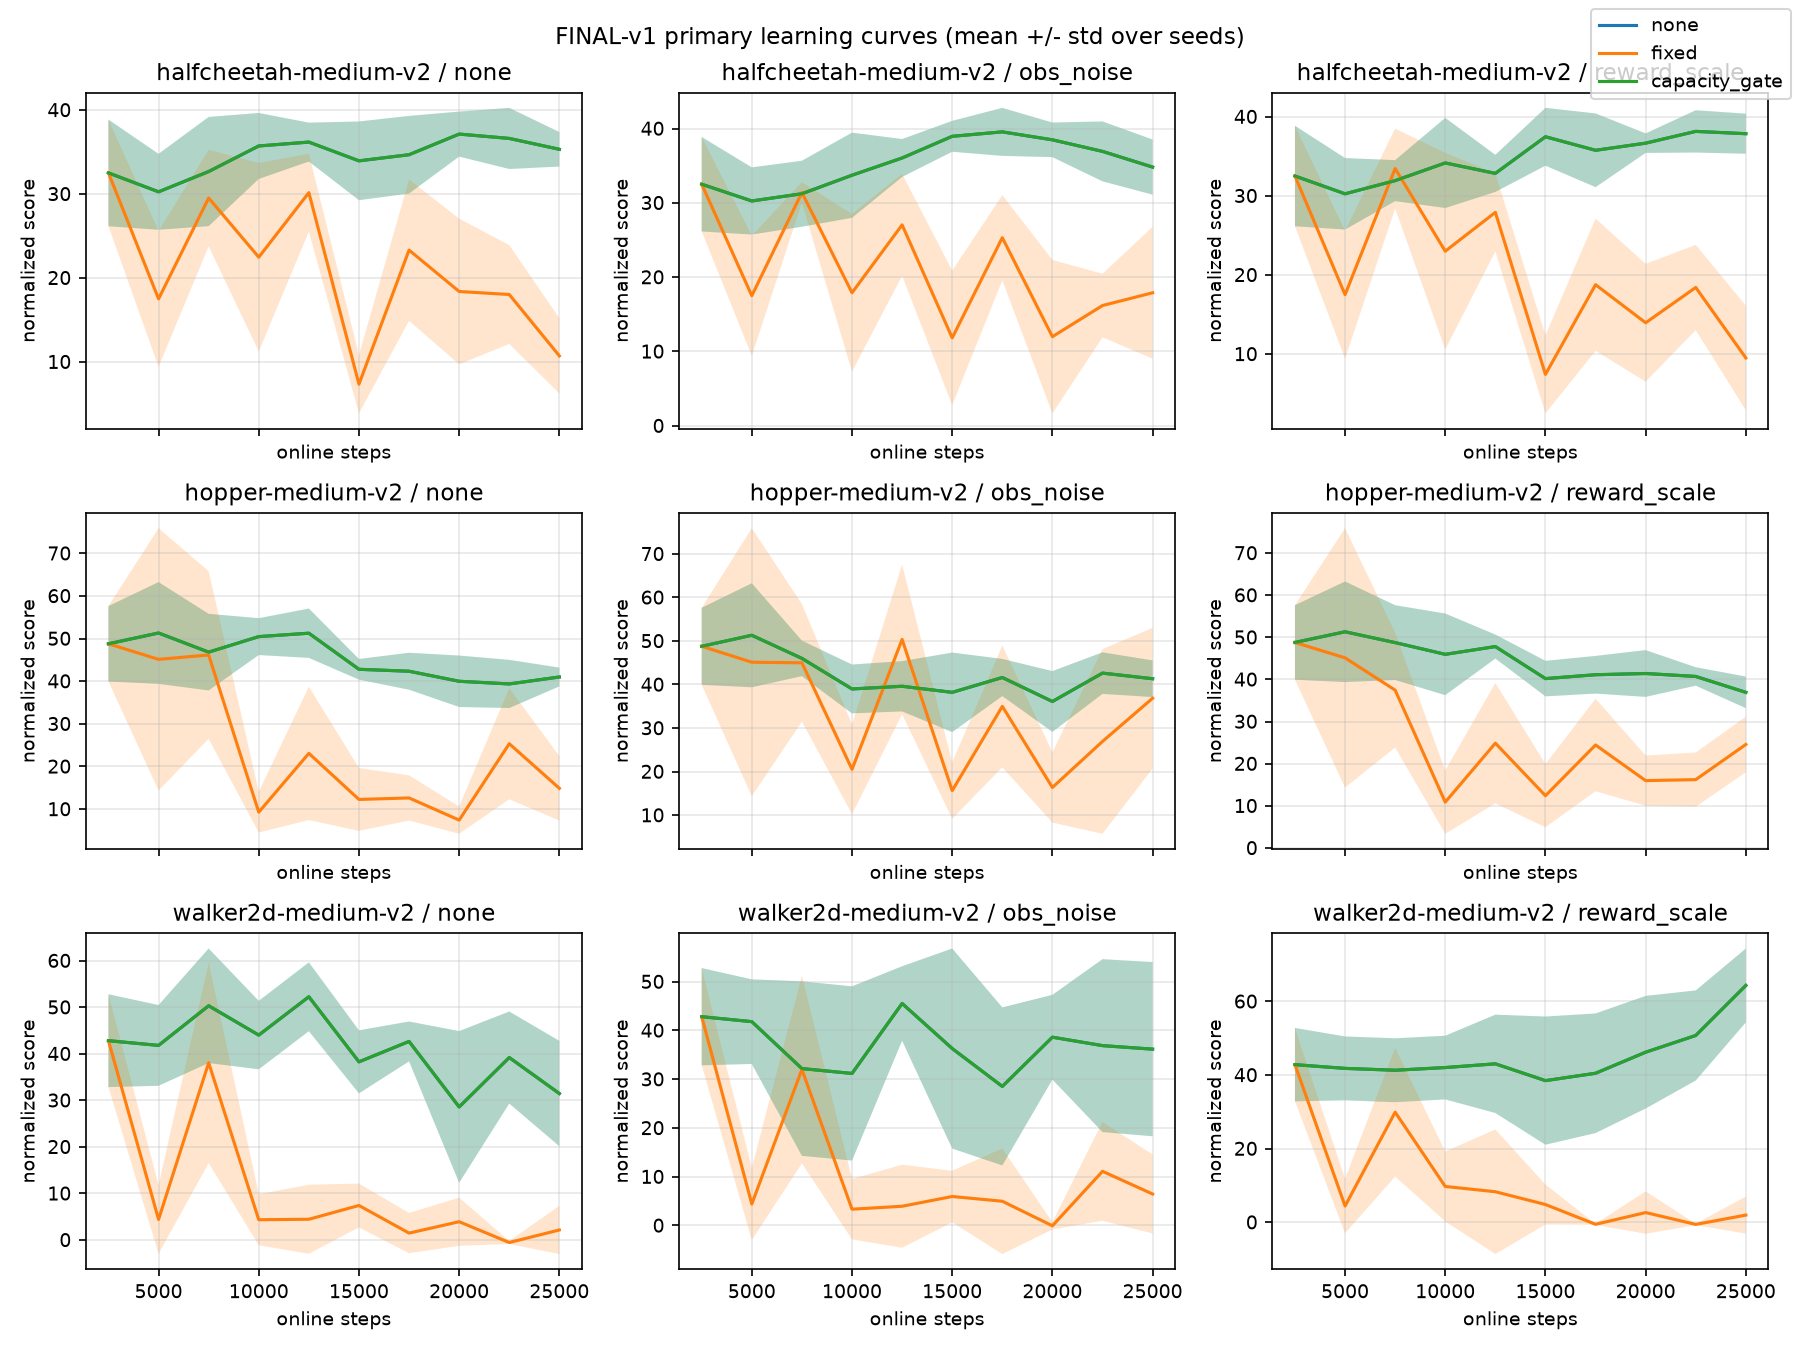
\includegraphics[width=0.96\textwidth]{figures/learning_curves.png}
\caption{\textbf{Online Adaptation Learning Curves Across 25,000 Fine-Tuning Steps.} Solid curves display mean evaluation normalized returns across 5 paired random seeds; shaded regions depict standard deviation. In balance-critical continuous-control locomotion (Hopper and Walker2d), periodic Shrink-and-Perturb induces immediate, unrecoverable policy failure. \textsc{CapacityGate} preserves baseline trajectories identically across all cells.}
\label{fig:learning_curves}
\end{figure}

\textbf{Aggregate Statistical Distribution.} Across all evaluated runs, aggregate IQM normalized returns demonstrate severe performance collapse under unconditional periodic Shrink-and-Perturb: Baseline (\texttt{none}) achieves $\mathrm{IQM} = 38.78$ ($95\%$ CI $[37.43, 40.03]$), Fixed Periodic (\texttt{fixed}) collapses to $\mathrm{IQM} = 12.30$ ($95\%$ CI $[9.36, 15.10]$), and \textsc{CapacityGate} matches Baseline at $\mathrm{IQM} = 38.78$. A paired Wilcoxon signed-rank test on $(\text{Baseline} - \text{Fixed})$ across all $N=45$ matched primary pairs confirms a decisive penalty for unconditional intervention ($W = 18.0$, $p = 1.44 \times 10^{-11}$; paired $t$-test $t = 9.15, p = 9.69 \times 10^{-12}$). Baseline outperforms Fixed in 42 of 45 pairs (93.3\%), with a mean paired difference of $+26.03 \pm 19.09$ (95\% bootstrap CI $[20.72, 31.59]$) and median $+22.27$. The empirical probability of improvement is $P(\text{None} > \text{Fixed}) = 0.933$ ($P(\text{Fixed} > \text{None}) = 0.067$, Figure~\ref{fig:aggregate_benchmark}b).

\textbf{Task-Specific Sensitivity.} In balance-critical Walker2d, periodic intervention drops clean return from $31.45 \pm 12.65$ to $2.14 \pm 5.79$, and reward-scaled return from $64.33 \pm 11.22$ to $1.94 \pm 5.64$, as weight noise repeatedly destroys the dynamic bipedal limit cycle. On Hopper, Fixed degrades clean return from $40.98 \pm 2.46$ to $14.87 \pm 8.45$. Even in unconstrained HalfCheetah, return drops from $35.32 \pm 2.29$ to $10.71 \pm 5.02$ without exploratory gain (Figure~\ref{fig:learning_curves}).

\subsection{Diagnostic Abstention: Gating as a Policy Guardian}
\label{sec:abstention}

Throughout online adaptation in stable and moderately shifted regimes, representation capacity remains intact: relative effective rank remains stable ($\rho(t) \in [0.99, 1.03]$ vs. trigger threshold $\rho_{\mathrm{on}} = 0.70$), and dormant neuron fractions remain minimal ($d(t) \in [4.3\%, 8.5\%]$ vs. trigger threshold $d_{\mathrm{on}} = 0.15$). Consequently, \textsc{CapacityGate} records \textbf{zero observed interventions across all 45 primary cells in tested stable-transfer conditions} (0 triggers out of 1,125 periodic evaluations). By abstaining from unneeded mutation, \textsc{CapacityGate} preserves baseline normalized returns identically ($38.78$ IQM). This confirms that \emph{abstention is an active protective mechanism}: representations do not spontaneously collapse in stable O2O transfer, validating the ``Do Not Disturb'' principle (full trajectories and cross-regime distributions detailed in Appendix Figure~\ref{fig:capacity_trajectories}).

\subsection{Operator Stability Asymmetry Under Non-Stationary Stress}
\label{sec:stress}

When an agent experiences genuine physical disruption (joint actuator disabled at step 5,000: \textbf{joint index 0} on \texttt{halfcheetah-medium-v2}, \textbf{joint index 2} on \texttt{walker2d-medium-v2}), intervention efficacy becomes \textbf{both shift-regime- and operator-dependent} (Figure~\ref{fig:stress_operator_asymmetry}, Table~\ref{tab:stress_results}):

\begin{figure}[t]
\centering
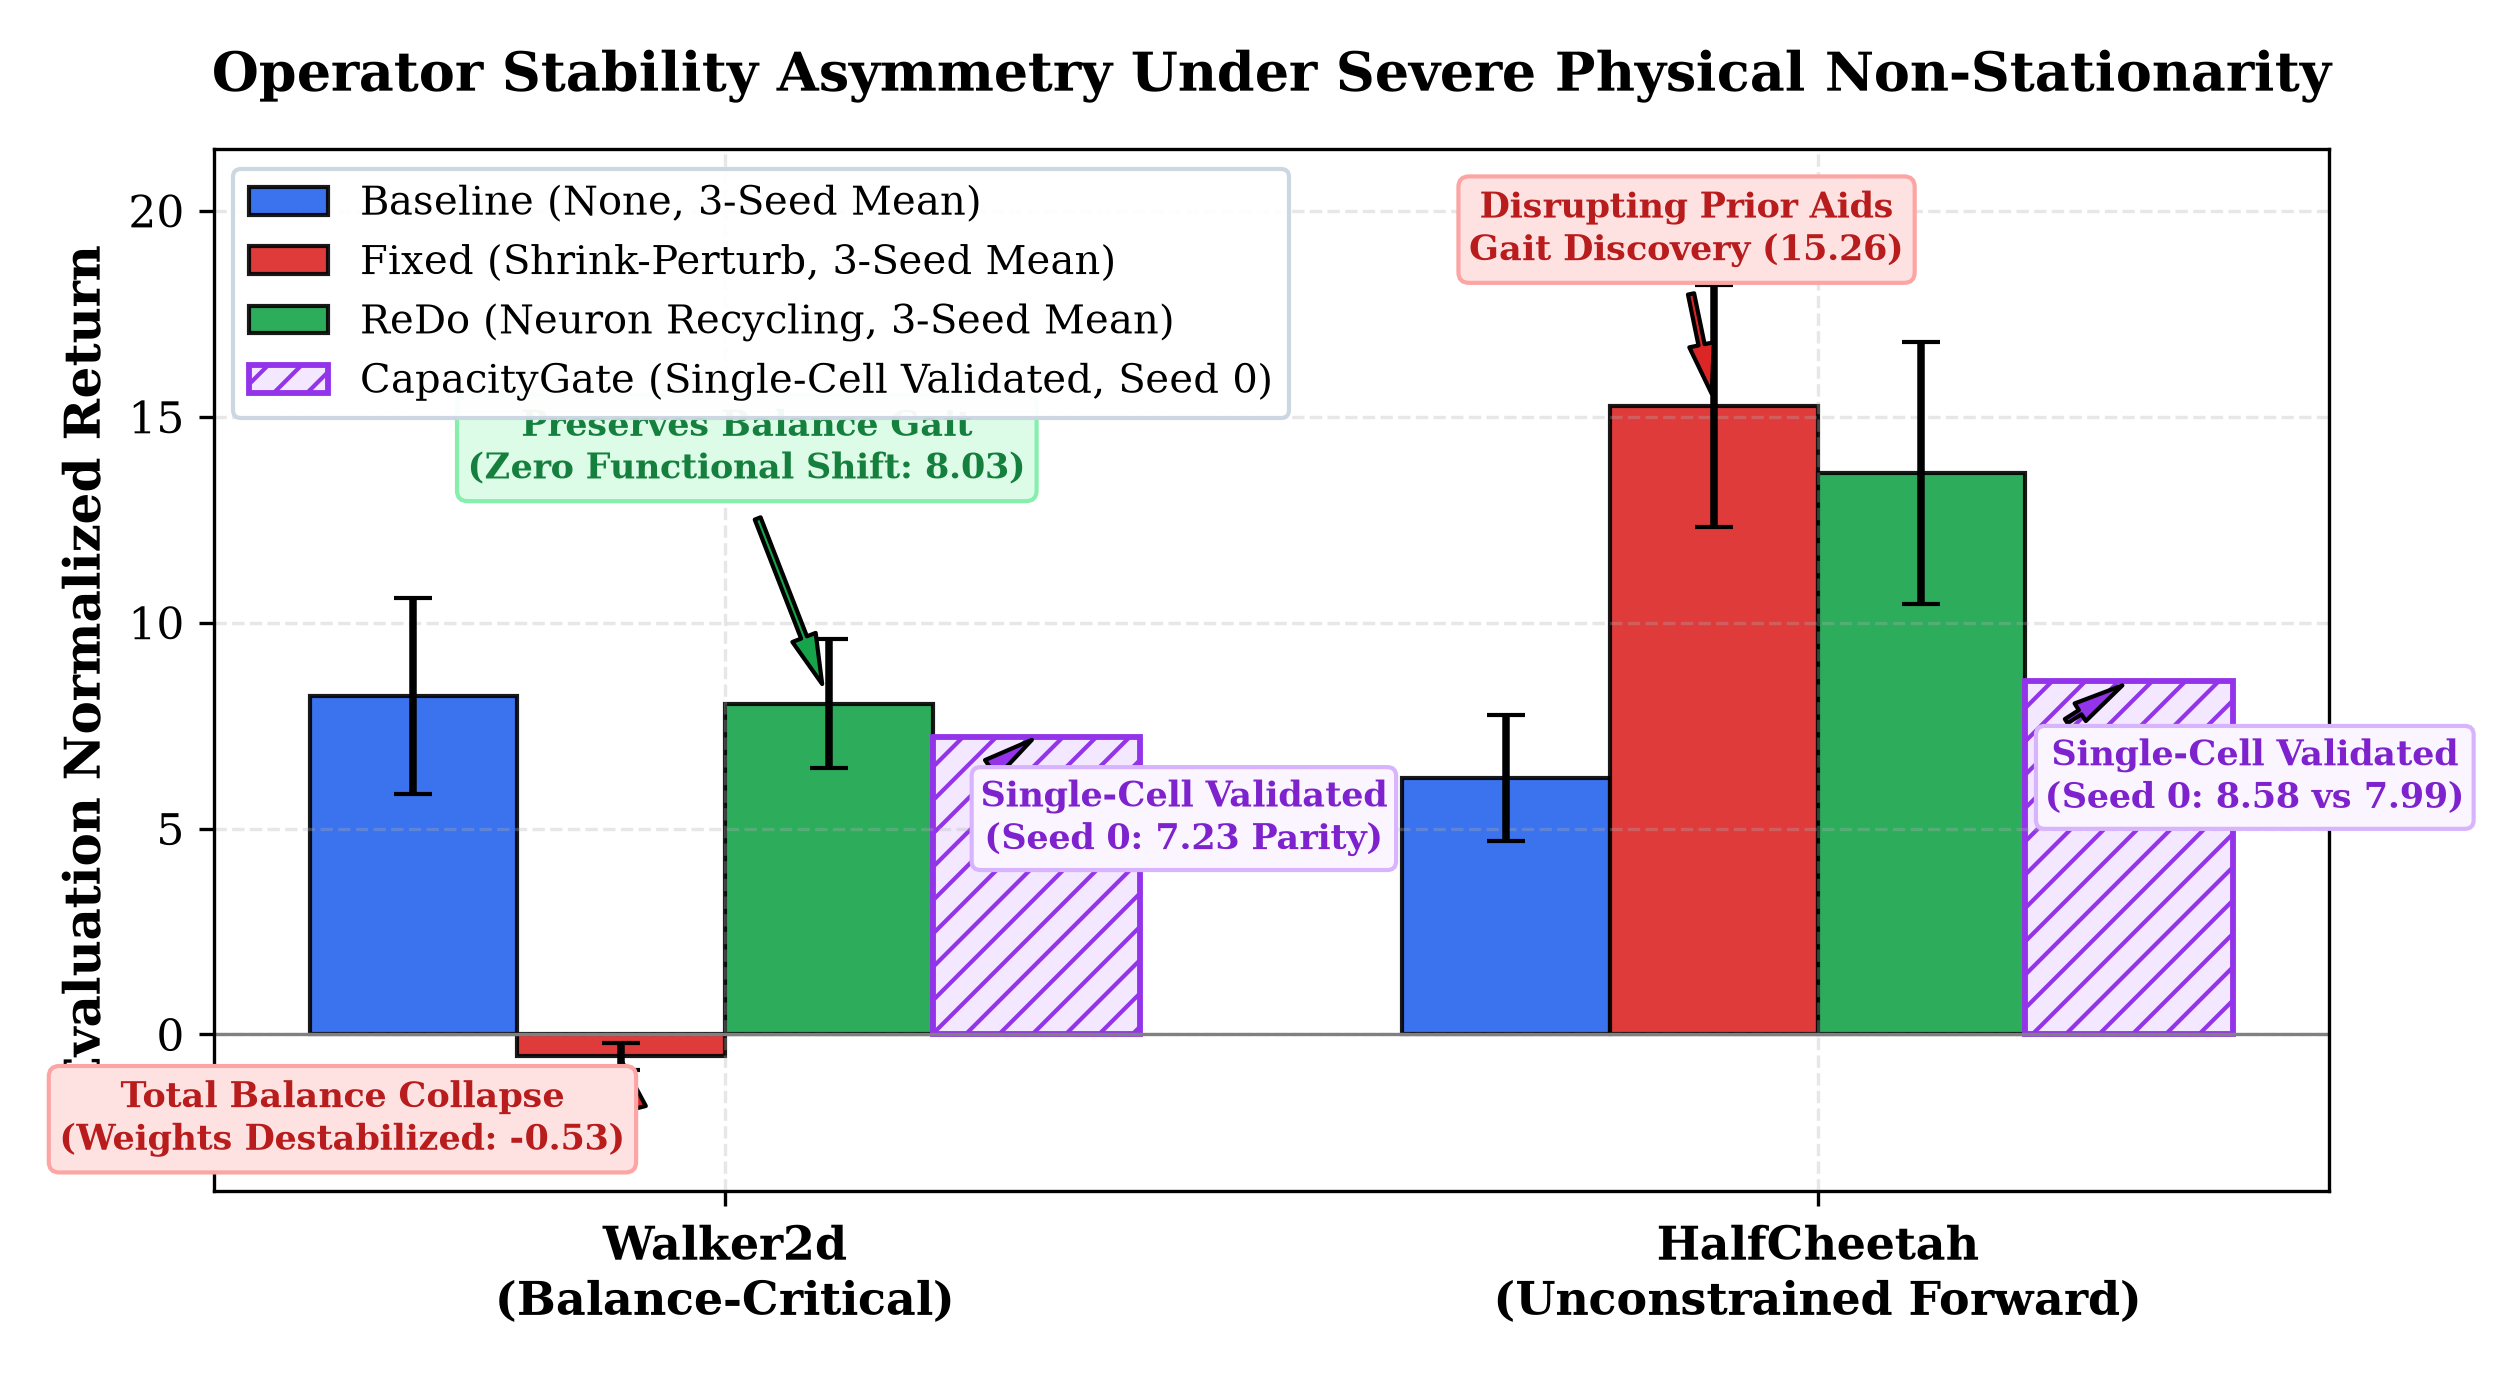
\includegraphics[width=0.88\textwidth]{figures/stress_operator_asymmetry.png}
\caption{\textbf{Operator Stability Asymmetry Under Physical Non-Stationarity.} Normalized returns under joint actuator crippling at step 5,000. Bars for Baseline (None), Fixed (Shrink-and-Perturb), and ReDo (Neuron Recycling) depict mean $\pm$ std across 3 paired seeds. CapacityGate is displayed with hatched bars to denote single-cell deterministic validation (Seed 0) rather than a 3-seed mean: on Walker2d Seed 0, CapacityGate safely abstains, preserving Baseline parity ($7.23$); on HalfCheetah Seed 0, it executes spaced pulses with refractory cooldown, achieving $8.58$ vs. $7.99$ unperturbed. In balance-critical Walker2d, weight-perturbation operators (Fixed) inject non-zero functional shifts that destroy the bipedal equilibrium manifold ($-0.53 \pm 0.33$). In sharp contrast, dormant neuron recycling (ReDo) preserves balance ($8.03 \pm 1.57$, matching Baseline $8.21 \pm 2.38$) due to its zero-functional-shift formulation ($W_{\mathrm{out}} = 0$). In unconstrained HalfCheetah, disrupting the offline prior aids in discovering alternate locomotion, enabling Fixed ($15.26 \pm 2.93$) and ReDo ($13.64 \pm 3.18$) to outperform the passive baseline ($6.23 \pm 1.53$).}
\label{fig:stress_operator_asymmetry}
\end{figure}

\begin{table}[t]
\caption{\textbf{Operator Stability Asymmetry Under Non-Stationary Stress.} Final evaluation normalized returns across 3 paired seeds under sudden actuator crippling ($a_{\mathrm{crippled}} = 0$ at step 5,000; joint 0 on HalfCheetah, joint 2 on Walker2d). On Walker2d, zero-functional-shift ReDo preserves bipedal locomotion ($8.03 \pm 1.57$), while weight perturbation (Fixed) destroys balance ($-0.53 \pm 0.33$).}
\label{tab:stress_results}
\centering
\small
\begin{tabular}{llcccc}
\toprule
\textbf{Environment} & \textbf{Arm} & \textbf{Seed 0} & \textbf{Seed 1} & \textbf{Seed 2} & \textbf{Mean $\pm$ Std} \\
\midrule
\multirow{4}{*}{\texttt{halfcheetah-medium-v2}} 
  & \texttt{none} & $7.99$ & $5.49$ & $5.21$ & $6.23 \pm 1.53$ \\
  & \texttt{fixed} (SP) & $15.29$ & $12.32$ & $18.18$ & $\mathbf{15.26} \pm \mathbf{2.93}$ \\
  & \texttt{redo} (Neuron Recycling) & $11.40$ & $12.25$ & $17.29$ & $13.64 \pm 3.18$ \\
  & \textsc{CapacityGate} & $8.58$ & --- & --- & $8.58$ (Single-Cell Validated) \\
\midrule
\multirow{4}{*}{\texttt{walker2d-medium-v2}} 
  & \texttt{none} & $7.23$ & $10.93$ & $6.48$ & $8.21 \pm 2.38$ \\
  & \texttt{fixed} (SP) & $-0.71$ & $-0.15$ & $-0.73$ & $-0.53 \pm 0.33$ \\
  & \texttt{redo} (Neuron Recycling) & $8.45$ & $9.34$ & $6.29$ & $\mathbf{8.03} \pm \mathbf{1.57}$ \\
  & \textsc{CapacityGate} (Seed 0 Abstain) & $7.23$ & --- & --- & $7.23$ (Baseline Parity) \\
\bottomrule
\end{tabular}
\end{table}

\textbf{Walker2d Balance Collapse (Fixed $-0.53$ vs. ReDo $8.03$ vs. Baseline $8.21$).} Walker2d requires continuous bipedal coordination. Shrink-and-Perturb injects non-zero functional shifts ($\Delta f_\theta(x) \neq 0$), collapsing return to $-0.53 \pm 0.33$. In stark contrast, ReDo recycles dormant neurons with outgoing weights zeroed ($W_{\mathrm{out}} = 0$), preserving input-output mappings identically ($f_{\theta'}(x) \equiv f_\theta(x)$) and maintaining viable walking dynamics ($8.03 \pm 1.57$, matching Baseline $8.21 \pm 2.38$).

\textbf{HalfCheetah Gait Adaptation (Fixed $15.26$ vs. ReDo $13.64$ vs. Baseline $6.23$).} Disabling the rear actuator (joint 0) impedes forward velocity under the offline prior ($6.23 \pm 1.53$). In this forward propulsion task where falling is impossible, empirical observations indicate that disrupting the offline prior via weight perturbation or neuron recycling is consistent with discovering alternate front-joint locomotion modes, enabling Fixed ($15.26 \pm 2.93$) and ReDo ($13.64 \pm 3.18$) to outperform the passive baseline.

\subsection{Controller Dynamics: Diagnostic Causality and Refractory Spacing}
\label{sec:telemetry}

Step-by-step diagnostic telemetry under actuator crippling on \texttt{halfcheetah-medium-v2} (Seed 0; full trace in Appendix Table~\ref{tab:telemetry_audit}) confirms the causal mechanics of \textsc{CapacityGate}. Pre-shift adaptation (steps 1,000--4,000) shows quiescent stability ($d = 0.043, \rho \in [0.85, 0.98]$), keeping the gate strictly dormant ($g_t = 0$). Post-shift joint crippling at step 5,000 causes rank decay, breaching the trigger threshold at step 7,000 ($\rho = 0.6948 \le 0.70$) and causally triggering intervention ($\|\Delta \theta\|_2 = 2.954$). The 3,000-step refractory cooldown spaces actuations (steps 7k, 10k, 13k, 16k, 19k, 22k). At step 25,000, intervention is intentionally skipped prior to final evaluation rollouts (\texttt{online\_step < online\_steps}), yielding a final evaluation return of $8.58$ (vs. $7.99$ unperturbed baseline).

\section{Discussion: Rethinking Plasticity in Transfer RL}
\label{sec:discussion}

\textbf{Intervention Vulnerability in Structured Control.} In offline-to-online continuous control, the primary hazard during online transfer is not the loss of plasticity, but the collateral destruction inflicted by interventions intended to restore it. Continuous locomotion manifolds occupy a narrow, coordinated subspace where balance and momentum are tightly coupled. Perturbing network weights by 10\% disrupts this dynamic equilibrium, causing unrecoverable falling and value divergence.

\textbf{The Plasticity vs. Adaptation Gap.} Representation capacity is a prerequisite, but not a guarantee, for policy adaptation. Restoring effective rank or recycling dead units provides the network with parameter degrees of freedom, but discovering viable gaits under altered kinematics requires directed exploration in state-action space. Capacity interventions cannot by themselves solve the exploration challenge.

\textbf{The ``Do Not Disturb'' Interpretation.} Rather than scheduling interventions open-loop (e.g., every $K$ steps), closed-loop capacity gating acts as an active circuit-breaker: when representations are healthy, leaving policy manifolds undisturbed is the safest and most effective strategy.

\section{Limitations}
\label{sec:limitations}

(1) \textbf{Locomotion Focus}: While D4RL represents the standard O2O continuous-control benchmark, evaluation in high-dimensional manipulation or vision-based RL warrants future exploration.
(2) \textbf{Exploration Independence}: \textsc{CapacityGate} acts on representation capacity; when distribution shifts require discovering disjoint behaviors, coupling gating with exploration is essential.
(3) \textbf{Hysteresis Calibration}: Deactivation thresholds must account for baseline dormancy ($7\text{--}12\%$ in active networks) to prevent latching.

\section{Conclusion and Future Work}
\label{sec:conclusion}

Across 150 total benchmark runs (135 primary factorial runs yielding $N = 45$ seed-matched comparisons, plus 15 reference runs) in offline-to-online continuous control, periodic Shrink-and-Perturb induces severe intervention vulnerability, causing a 68.3\% collapse in aggregate IQM return. We formulated the ``Do Not Disturb'' principle and introduced \textsc{CapacityGate}, demonstrating that closed-loop diagnostic abstention shields converged policies from unnecessary perturbation. Under actuator crippling, intervention operators exhibit a stark stability asymmetry: zero-functional-shift recycling (ReDo) preserves balance where weight perturbation collapses. Plasticity interventions should not be treated as blind background routines, but as regime- and operator-dependent operations governed by capacity telemetry.

\paragraph{Future Work}
Promising directions include:
(1) \textbf{Exploration-Oriented Zero-Shift Operators}: Combining the structural safety of zero-functional-shift recycling ($W_{\mathrm{out}} = 0$) with targeted exploratory policy perturbations to discover alternate kinematic gaits.
(2) \textbf{Multi-Timescale Adaptive Telemetry}: Extending \textsc{CapacityGate} to multi-agent and non-stationary competitive environments using streaming singular value updates.
(3) \textbf{Cross-Domain Plasticity Gating}: Applying capacity-gated abstention to foundation decision models and continuous real-to-sim transfer.

\subsubsection*{Reproducibility Statement}
All algorithmic mechanisms (\textsc{CapacityGate}), environment configurations, offline dataset specifications, hyperparameters (Table~\ref{tab:hyperparams}), and statistical evaluation protocols are detailed in Sections~\ref{sec:method} and~\ref{sec:setup} and the supplementary appendices. Full experimental source code, raw paired evaluation logs across all 150 benchmark runs, random seeds, and plotting scripts are included in the supplementary repository archive.

\subsubsection*{Use of AI Assistance}
During the preparation of this manuscript, large language models and AI tools were used for research ideation and exploratory execution, scientific literature retrieval and discovery, drafting portions of the manuscript, and writing and editing assistance. The authors critically reviewed, audited, and verified all AI-assisted material against the underlying empirical records and code, and take full responsibility for the final paper, experiments, mathematical formulations, claims, and conclusions.

\bibliography{iclr2027_conference}
\bibliographystyle{iclr2027_conference}

\newpage
\appendix

\section{Literature Comparison Matrix}
\label{app:lit_matrix}

Table~\ref{tab:lit_comparison} provides an extended conceptual and methodological comparison between \textsc{CapacityGate} and representative plasticity, reset, and transfer RL methods.

\begin{table}[h]
\caption{\textbf{Conceptual and Methodological Comparison with Prior Literature.}}
\label{tab:lit_comparison}
\centering
\scriptsize
\begin{tabular}{p{0.18\textwidth}p{0.16\textwidth}p{0.14\textwidth}p{0.14\textwidth}p{0.18\textwidth}p{0.14\textwidth}}
\toprule
\textbf{Method} & \textbf{Intervention Type} & \textbf{Trigger Mechanism} & \textbf{Evaluated Domain} & \textbf{Primary Objective} & \textbf{Key Vulnerability / Limitation} \\
\midrule
Resetting \newline \citep{nikishin2022primacy} & Complete/Penultimate Weight Reset & Open-loop \newline (Fixed $K$ steps) & Online RL (Atari, Gym) & Overcome primacy bias in tabula rasa RL & Erases learned representations; fatal for O2O transfer. \\
\midrule
Shrink-Perturb \newline \citep{ash2020warmstarting} & Weight Shrinkage + Gaussian Noise & Open-loop \newline (Fixed interval) & Continual Supervised Learning & Escape spurious local minima & Injects non-zero functional shift; destabilizes control. \\
\midrule
ReDo \newline \citep{sokar2023dormant} & Dormant Neuron Recycling & Open-loop \newline (Fixed interval) & Online RL (Atari) & Restore representation capacity via dead units & Evaluated only with periodic open-loop schedule. \\
\midrule
DR3 \newline \citep{kumar2022dr3} & Explicit Representation Regularizer & Implicit \newline (Continuous Loss) & Offline RL (D4RL) & Prevent feature rank collapse during pretraining & Passive penalty; cannot actively intervene online. \\
\midrule
\textbf{This Work} \newline (\textsc{CapacityGate}) & Closed-loop Gated Intervention & Closed-loop \newline ($\rho(t)$ and $d(t)$) & D4RL O2O continuous control & Introduces the ``Do Not Disturb'' principle; couples rank and dormancy. & Demonstrates that diagnostic abstention protects converged policies; reveals operator asymmetry. \\
\bottomrule
\end{tabular}
\end{table}

\section{Exhaustive Seed-Level Benchmark Data}
\label{app:per_seed}

Table~\ref{tab:per_seed_full} provides the complete, unabridged breakdown of final evaluation normalized returns across all 135 primary factorial runs in the confirmatory study, reporting individual performance for each of the 5 paired random seeds (Seeds 0--4).

\begin{table}[h]
\caption{\textbf{Complete 135-Run Primary Benchmark Breakdown.} Final evaluation normalized returns across all 5 paired random seeds (Seeds 0--4) for each (Environment, Shift Regime, Method) experimental cell, matching Table~\ref{tab:main_results} exactly.}
\label{tab:per_seed_full}
\centering
\scriptsize
\begin{tabular}{lllccccc}
\toprule
\textbf{Environment} & \textbf{Shift Regime} & \textbf{Method} & \textbf{Seed 0} & \textbf{Seed 1} & \textbf{Seed 2} & \textbf{Seed 3} & \textbf{Seed 4} \\
\midrule
\multirow{9}{*}{\texttt{halfcheetah-medium-v2}}
 & \multirow{3}{*}{\texttt{none}}
   & \texttt{none} & $38.23$ & $35.96$ & $35.36$ & $35.21$ & $31.83$ \\
   & \texttt{fixed} & $16.33$ & $11.82$ & $12.19$ & $10.58$ & $2.61$ \\
   & \textsc{CapacityGate} & $38.23$ & $35.96$ & $35.36$ & $35.21$ & $31.83$ \\
 \cmidrule{2-8}
 & \multirow{3}{*}{\texttt{obs\_noise}}
   & \texttt{none} & $32.83$ & $29.78$ & $38.16$ & $39.92$ & $33.37$ \\
   & \texttt{fixed} & $17.52$ & $29.75$ & $20.78$ & $19.10$ & $2.30$ \\
   & \textsc{CapacityGate} & $32.83$ & $29.78$ & $38.16$ & $39.92$ & $33.37$ \\
 \cmidrule{2-8}
 & \multirow{3}{*}{\texttt{reward\_scale}}
   & \texttt{none} & $38.00$ & $35.27$ & $41.55$ & $39.56$ & $34.88$ \\
   & \texttt{fixed} & $16.32$ & $5.33$ & $1.83$ & $18.45$ & $5.54$ \\
   & \textsc{CapacityGate} & $38.00$ & $35.27$ & $41.55$ & $39.56$ & $34.88$ \\
 \midrule
\multirow{9}{*}{\texttt{hopper-medium-v2}}
 & \multirow{3}{*}{\texttt{none}}
   & \texttt{none} & $39.98$ & $37.49$ & $43.99$ & $42.38$ & $41.08$ \\
   & \texttt{fixed} & $20.07$ & $16.31$ & $10.12$ & $24.69$ & $3.14$ \\
   & \textsc{CapacityGate} & $39.98$ & $37.49$ & $43.99$ & $42.38$ & $41.08$ \\
 \cmidrule{2-8}
 & \multirow{3}{*}{\texttt{obs\_noise}}
   & \texttt{none} & $47.66$ & $37.05$ & $37.52$ & $39.56$ & $44.84$ \\
   & \texttt{fixed} & $55.16$ & $24.04$ & $28.10$ & $19.46$ & $57.47$ \\
   & \textsc{CapacityGate} & $47.66$ & $37.05$ & $37.52$ & $39.56$ & $44.84$ \\
 \cmidrule{2-8}
 & \multirow{3}{*}{\texttt{reward\_scale}}
   & \texttt{none} & $41.95$ & $33.50$ & $39.85$ & $31.95$ & $37.38$ \\
   & \texttt{fixed} & $19.73$ & $17.81$ & $21.69$ & $27.53$ & $36.03$ \\
   & \textsc{CapacityGate} & $41.95$ & $33.50$ & $39.85$ & $31.95$ & $37.38$ \\
 \midrule
\multirow{9}{*}{\texttt{walker2d-medium-v2}}
 & \multirow{3}{*}{\texttt{none}}
   & \texttt{none} & $9.97$ & $38.71$ & $33.62$ & $42.43$ & $32.54$ \\
   & \texttt{fixed} & $12.48$ & $-0.69$ & $-0.04$ & $-0.45$ & $-0.60$ \\
   & \textsc{CapacityGate} & $9.97$ & $38.71$ & $33.62$ & $42.43$ & $32.54$ \\
 \cmidrule{2-8}
 & \multirow{3}{*}{\texttt{obs\_noise}}
   & \texttt{none} & $1.45$ & $41.90$ & $40.01$ & $45.02$ & $52.41$ \\
   & \texttt{fixed} & $-0.25$ & $19.62$ & $1.26$ & $12.18$ & $-0.56$ \\
   & \textsc{CapacityGate} & $1.45$ & $41.90$ & $40.01$ & $45.02$ & $52.41$ \\
 \cmidrule{2-8}
 & \multirow{3}{*}{\texttt{reward\_scale}}
   & \texttt{none} & $61.16$ & $66.03$ & $47.08$ & $76.66$ & $70.71$ \\
   & \texttt{fixed} & $-0.74$ & $12.03$ & $-0.55$ & $-0.50$ & $-0.52$ \\
   & \textsc{CapacityGate} & $61.16$ & $66.03$ & $47.08$ & $76.66$ & $70.71$ \\
\bottomrule
\end{tabular}
\end{table}

\newpage
\section{Diagnostic Parameter Specifications}
\label{app:hyperparams}

Table~\ref{tab:hyperparams} specifies the primary hyperparameters governing offline pretraining, online adaptation, diagnostic probe evaluation, and \textsc{CapacityGate} controller execution.

\begin{table}[h]
\caption{\textbf{Experimental Hyperparameters and Diagnostic Settings.}}
\label{tab:hyperparams}
\centering
\small
\begin{tabular}{ll}
\toprule
\textbf{Hyperparameter} & \textbf{Setting / Value} \\
\midrule
Offline Pretraining Updates & $25,000$ \\
Online Adaptation Steps & $25,000$ \\
Offline Replay Ratio & $0.50$ ($50\%$ offline, $50\%$ online) \\
Online Update Frequency & $1$ update per environment step \\
Batch Size & $256$ \\
IQL Temperature ($\beta$) & $3.0$ \\
IQL Expectile ($\tau$) & $0.70$ \\
Discount Factor ($\gamma$) & $0.99$ \\
Target Network Polyak Factor & $0.005$ \\
Optimizer & Adam ($\mathrm{lr} = 3 \times 10^{-4}$) \\
Optimizer Moment Reset & $m_t \leftarrow 0, v_t \leftarrow 0$ upon parameter intervention \\
Diagnostic Probe Interval ($\Delta t$) & $1,000$ steps \\
Probe Batch Size ($B$) & $256$ (Uniform Replay Reservoir) \\
Effective Rank Ratio Trigger ($\rho_{\mathrm{on}}$) & $0.70$ ($70\%$ baseline capacity) \\
Effective Rank Ratio Recovery ($\rho_{\mathrm{off}}$) & $0.85$ ($85\%$ baseline capacity) \\
Dormancy On Threshold ($d_{\mathrm{on}}$) & $0.15$ ($15\%$ dormant units) \\
Dormancy Off Threshold ($d_{\mathrm{off}}$) & $0.08$ ($8\%$ dormant units) \\
Refractory Cooldown ($\Delta_{\mathrm{cool}}$) & $3,000$ steps \\
Terminal Step Policy & Bypass intervention at $t = 25,000$ prior to rollout \\
Perturbation Severity ($\sigma$) & $0.10$ \\
Perturbation Shrink Factor ($\lambda$) & $0.10$ \\
ReDo Activation Threshold ($\tau_{\mathrm{redo}}$) & $0.10$ \\
\bottomrule
\end{tabular}
\end{table}

\section{Diagnostic Telemetry Trajectories Across Regimes}
\label{app:telemetry_plots}

Figure~\ref{fig:capacity_trajectories} displays live online diagnostic trajectories for relative effective rank ($\rho$) and activation dormancy ($d$) across clean and shifted adaptation, as well as performance retention distributions.

\begin{figure}[h]
\centering
\begin{subfigure}[b]{0.48\textwidth}
    \centering
    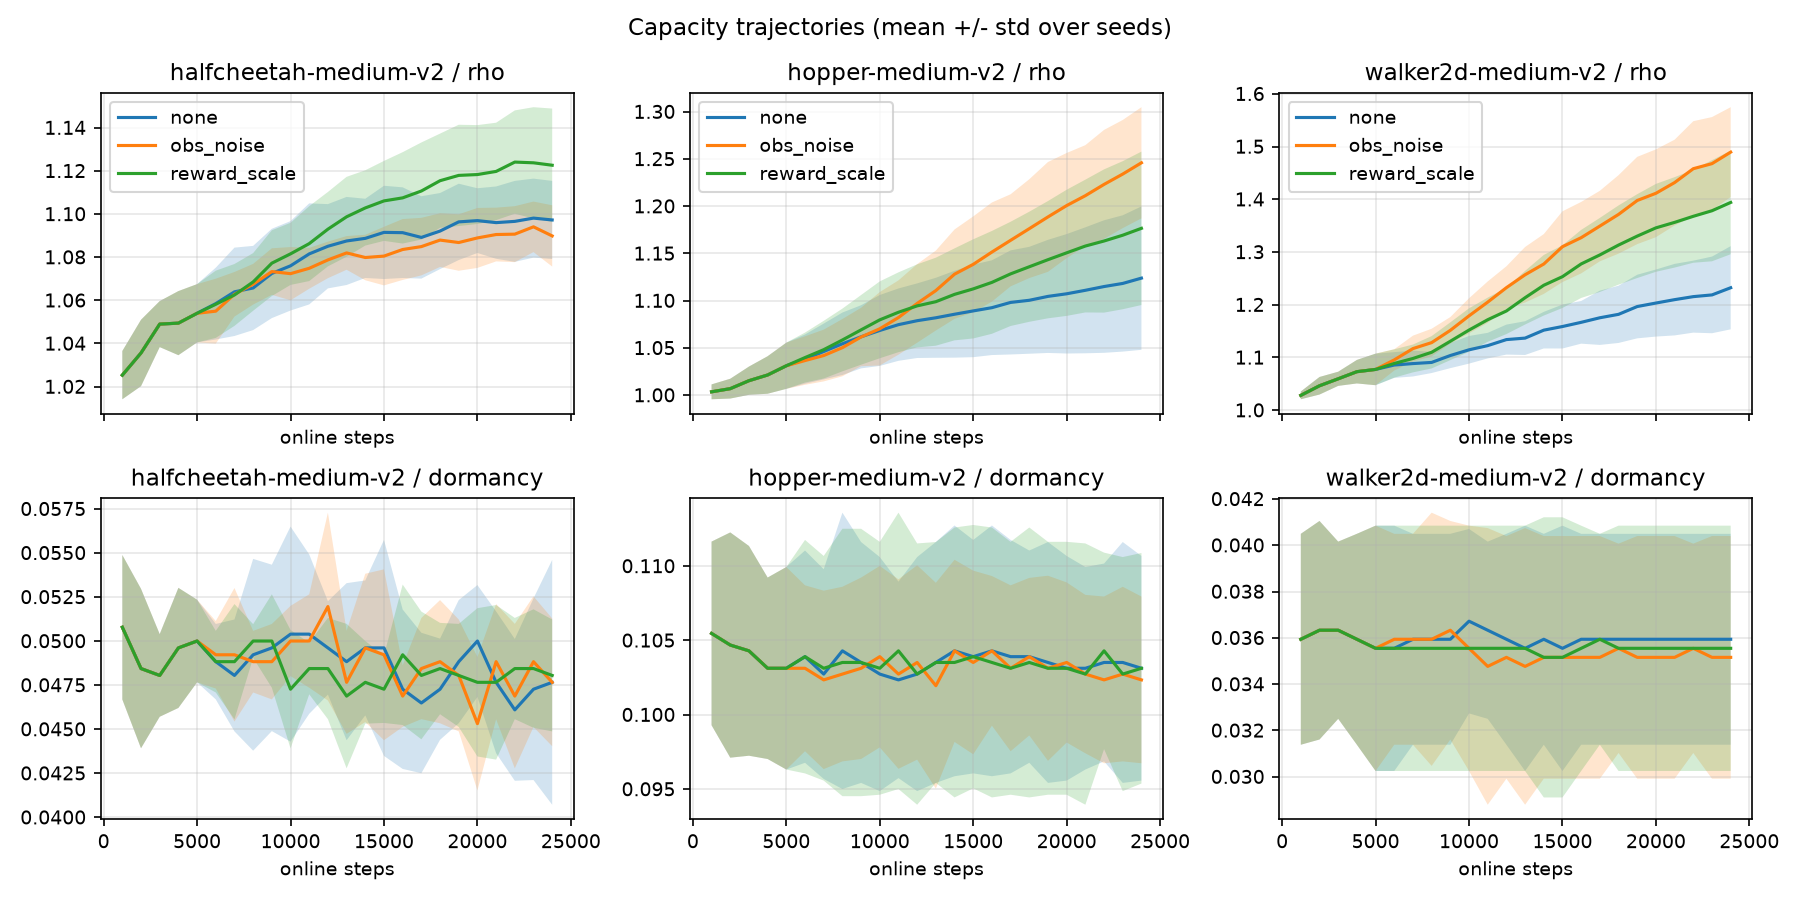
\includegraphics[width=\textwidth]{figures/capacity_trajectories.png}
    \caption{Diagnostic Telemetry Trajectories}
    \label{fig:telemetry_trajectories_app}
\end{subfigure}
\hfill
\begin{subfigure}[b]{0.48\textwidth}
    \centering
    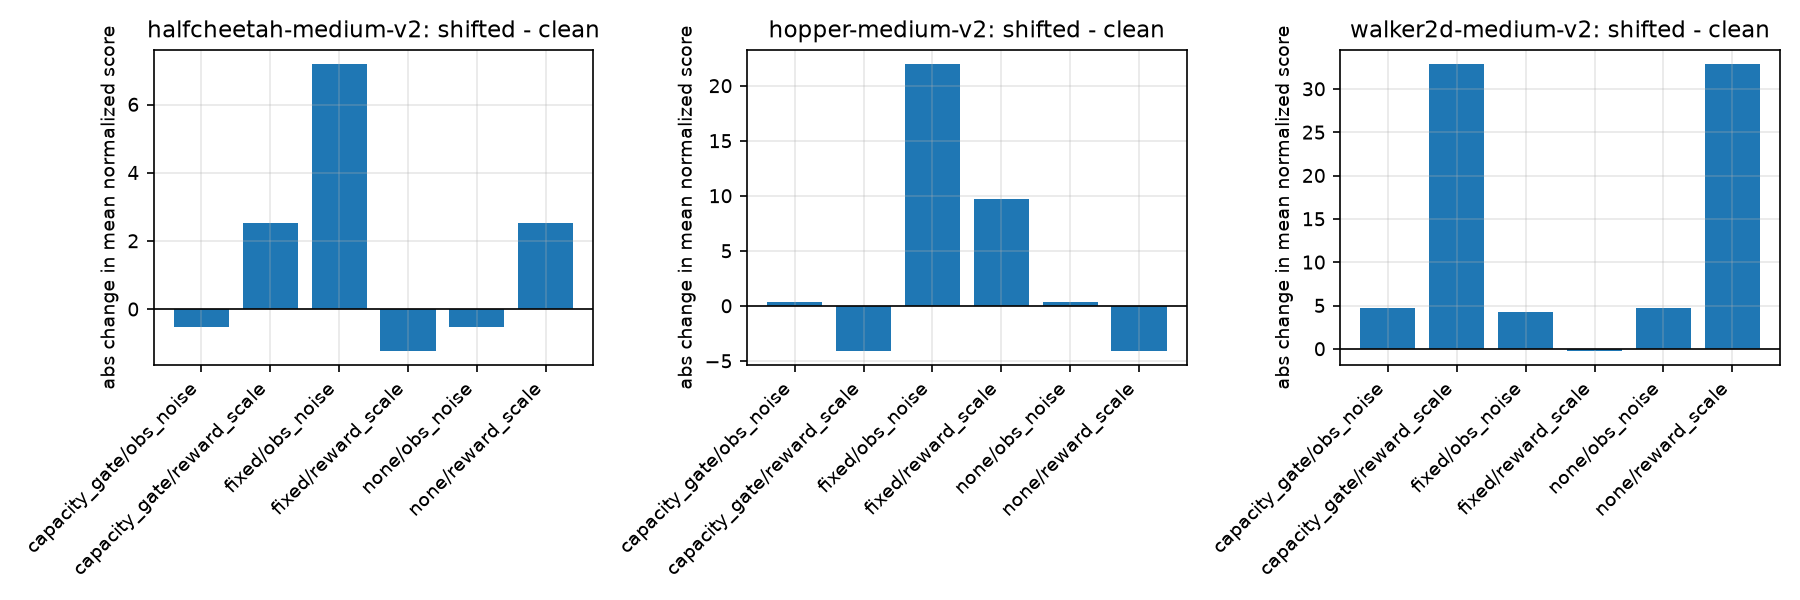
\includegraphics[width=\textwidth]{figures/clean_vs_shifted.png}
    \caption{Performance Retention Across Regimes}
    \label{fig:clean_vs_shifted_app}
\end{subfigure}
\caption{\textbf{Diagnostic Telemetry and Cross-Regime Performance Retention.} (a) Online trajectories of relative effective rank ($\rho$) and activation dormancy ($d$) under clean and shifted regimes. Representation capacity remains well within healthy operational bounds ($\rho > 0.70, d < 0.15$). (b) Normalized returns across clean, observation noise, and reward scaling regimes: \textsc{CapacityGate} matches Baseline across all regimes, avoiding the collapse of unconditional intervention.}
\label{fig:capacity_trajectories}
\end{figure}

\newpage
\section{Step-by-Step Diagnostic Telemetry Trace Under Actuator Stress}
\label{app:telemetry_trace}

Table~\ref{tab:telemetry_audit} documents the complete step-by-step diagnostic telemetry progression on \texttt{halfcheetah-medium-v2} (Seed 0, Actuator Crippling at step 5,000; joint index 0), verifying pre-shift quiescence, causal activation upon rank collapse at step 7,000, refractory-spaced actuations, and intentional terminal intervention bypass at step 25,000.

\begin{table}[h]
\caption{\textbf{Step-by-Step Diagnostic Telemetry Under Actuator Crippling.} Validated telemetry on \texttt{halfcheetah-medium-v2} (Seed 0, Actuator Cripple at step 5,000) using uniform probe sampling, cooldown $\Delta_{\mathrm{cool}} = 3,000$ steps, and decoupled severity $\eta = 0.1$. Parameter intervention is bypassed at terminal step 25,000 (\texttt{online\_step < online\_steps}) prior to evaluation rollouts.}
\label{tab:telemetry_audit}
\centering
\scriptsize
\begin{tabular}{rcccccccc}
\toprule
\textbf{Step} & \textbf{Shift Active} & \textbf{Gate State} & \textbf{Intervene} & \textbf{Cooldown} & \textbf{Dormancy ($d$)} & \textbf{Rank Ratio ($\rho$)} & \textbf{$\|\Delta \theta\|_2$} & \textbf{Controller State} \\
\midrule
1,000 & False & False & False & False & $0.0430$ & $0.8474$ & $0.000$ & Nominal / Quiescent \\
2,000 & False & False & False & False & $0.0430$ & $0.9288$ & $0.000$ & Nominal / Quiescent \\
3,000 & False & False & False & False & $0.0430$ & $0.9836$ & $0.000$ & Nominal / Quiescent \\
4,000 & False & False & False & False & $0.0430$ & $0.8595$ & $0.000$ & Nominal / Quiescent \\
\midrule
5,000 & \textbf{True} & False & False & False & $0.0469$ & $0.7719$ & $0.000$ & Physical Shift Begins \\
6,000 & True & False & False & False & $0.0410$ & $0.7044$ & $0.000$ & Pre-Trigger Degradation \\
\midrule
7,000 & True & \textbf{True} & \textbf{True} & False & $0.0391$ & $0.6948$ & $2.954$ & \textbf{Causal Trigger 1 ($\rho \le 0.70$)} \\
8,000 & True & True & False & \textbf{True} & $0.0508$ & $0.5885$ & $0.000$ & Refractory Cooldown \\
9,000 & True & True & False & \textbf{True} & $0.0449$ & $0.6002$ & $0.000$ & Refractory Cooldown \\
\midrule
10,000 & True & True & \textbf{True} & False & $0.0508$ & $0.5964$ & $2.899$ & \textbf{Actuation Pulse 2} \\
13,000 & True & True & \textbf{True} & False & $0.0469$ & $0.4757$ & $2.810$ & \textbf{Actuation Pulse 3} \\
16,000 & True & True & \textbf{True} & False & $0.0684$ & $0.3597$ & $2.761$ & \textbf{Actuation Pulse 4} \\
19,000 & True & True & \textbf{True} & False & $0.0859$ & $0.3308$ & $2.779$ & \textbf{Actuation Pulse 5} \\
22,000 & True & True & \textbf{True} & False & $0.0898$ & $0.2760$ & $2.761$ & \textbf{Actuation Pulse 6} \\
\midrule
25,000 & True & True & False & True & $0.0918$ & $0.2454$ & $0.000$ & Terminal Bypass: Return \textbf{8.58} (Baseline: 7.99) \\
\bottomrule
\end{tabular}
\end{table}

\end{document}
